
\documentclass[a4paper, 14pt]{extarticle}
% Поля
%--------------------------------------
\usepackage{geometry}
\geometry{a4paper,tmargin=2cm,bmargin=2cm,lmargin=3cm,rmargin=1cm}
%--------------------------------------


%Russian-specific packages
%--------------------------------------
\usepackage[T2A]{fontenc}
\usepackage[utf8]{inputenc} 
\usepackage[english, main=russian]{babel}

\usepackage{pgfplots}
\pgfplotsset{compat=1.9}

%--------------------------------------

\usepackage{textcomp}
\usepackage{comment}
\usepackage{array}
% Красная строка
%--------------------------------------
\usepackage{indentfirst}               
%--------------------------------------             


%Graphics
%--------------------------------------
\usepackage{graphicx}
\graphicspath{ {./images/} }
\usepackage{wrapfig}
%--------------------------------------

% Полуторный интервал
%--------------------------------------
\linespread{1.3}                    
%--------------------------------------

%Выравнивание и переносы
%--------------------------------------
% Избавляемся от переполнений
\sloppy
% Запрещаем разрыв страницы после первой строки абзаца
\clubpenalty=10000
% Запрещаем разрыв страницы после последней строки абзаца
\widowpenalty=10000
%--------------------------------------

%Списки
\usepackage{enumitem}

%Подписи
\usepackage{caption} 

%Гиперссылки
\usepackage{hyperref}

\hypersetup {
	unicode=true
}

%Рисунки
%--------------------------------------
\DeclareCaptionLabelSeparator*{emdash}{~--- }
\captionsetup[figure]{labelsep=emdash,font=onehalfspacing,position=bottom}
%--------------------------------------

\usepackage{tempora}
\usepackage{amsmath}
\usepackage{color}
\usepackage{listings}
\lstset{
  belowcaptionskip=1\baselineskip,
  breaklines=true,
  extendedchars=\true,
  inputencoding=utf8x,
  frame=L,
  xleftmargin=\parindent,
  language=Python,
  showstringspaces=false,
  basicstyle=\footnotesize\ttfamily,
  keywordstyle=\bfseries\color{blue},
  commentstyle=\itshape\color{purple},
  identifierstyle=\color{black},
  stringstyle=\color{red},
}

%--------------------------------------
%			НАЧАЛО ДОКУМЕНТА
%--------------------------------------

\begin{document}

%--------------------------------------
%			ТИТУЛЬНЫЙ ЛИСТ
%--------------------------------------
\begin{titlepage}
\thispagestyle{empty}
\newpage


%Шапка титульного листа
%--------------------------------------
\vspace*{-60pt}
\hspace{-65pt}
\begin{minipage}{0.3\textwidth}
\hspace*{-20pt}\centering
\includegraphics[width=\textwidth]{emblem.png}
\end{minipage}
\begin{minipage}{0.67\textwidth}\small \textbf{
\vspace*{-0.7ex}
\hspace*{-6pt}\centerline{Министерство науки и высшего образования Российской Федерации}
\vspace*{-0.7ex}
\centerline{Федеральное государственное бюджетное образовательное учреждение }
\vspace*{-0.7ex}
\centerline{высшего образования}
\vspace*{-0.7ex}
\centerline{<<Московский государственный технический университет}
\vspace*{-0.7ex}
\centerline{имени Н.Э. Баумана}
\vspace*{-0.7ex}
\centerline{(национальный исследовательский университет)>>}
\vspace*{-0.7ex}
\centerline{(МГТУ им. Н.Э. Баумана)}}
\end{minipage}
%--------------------------------------

%Полосы
%--------------------------------------
\vspace{0pt}
\hspace{-35pt}\rule{\textwidth}{2.3pt}

\vspace*{-20pt}
\hspace{-35pt}\rule{\textwidth}{0.4pt}
%--------------------------------------

\vspace{1ex}
\hspace{-35pt} \noindent \small ФАКУЛЬТЕТ\hspace{80pt} <<Информатика и системы управления>>

\vspace*{-16pt}
\hspace{47pt}\rule{0.83\textwidth}{0.4pt}

\vspace{0.5ex}
\hspace{-35pt} \noindent \small КАФЕДРА\hspace{50pt} <<Теоретическая информатика и компьютерные технологии>>

\vspace*{-16pt}
\hspace{30pt}\rule{0.866\textwidth}{0.4pt}
  
\vspace{11em}

\begin{center}
\Large {\bf Лабораторная работа № 2} \\ 
\large {\bf по курсу <<Теория формальных языков>>} \\ 
\end{center}\normalsize

\vspace{8em}


\begin{flushright}
  {Студент группы ИУ9-51Б Григорян Д. А.\hspace*{15pt} \\
  \vspace{2ex}
  Преподаватель Непейвода А. Н.\hspace*{15pt}}
\end{flushright}

\bigskip

\vfill
 

\begin{center}
\textsl{Москва 2025}
\end{center}
\end{titlepage}
%--------------------------------------
%		КОНЕЦ ТИТУЛЬНОГО ЛИСТА
%--------------------------------------


\renewcommand{\ttdefault}{pcr}

\setlength{\tabcolsep}{3pt}
\newpage
\setcounter{page}{2}
\section*{Задача}\label{Sect::task}
По имеющемуся академическому регулярному выражению построить:

\begin{itemize}
\item Минимальный ДКА, распознающий его язык (минимальность обосновать таблицей классов эквивалентности)

\item Возможно малый НКА, распознающий его язык. Возможно малый переключающийся (с конъюнкцией) КА, распознающий его язык. Частично обосновать таблицами множеств классов эквивалентности.

\item Расширенное регулярное выражение, распознающее тот же язык. В расширенном выражении можно использовать:

\begin{itemize}
\item wildcard-операцию . для замены произвольного символа алфавита;
\item положительную итерацию $\tau^+$ и опцию $\tau?$. $\tau^+ = \tau\tau^*$, $\tau? = (\tau|\varepsilon)$;
\item операции предпросмотра $\tau_0(?= \tau_1)\tau_2 \equiv \tau_0((\tau_1.*) \cap \tau_2)$ и ретроспективной проверки $\tau_0(?<= \tau_1)\tau_2 \equiv (\tau_0 \cap (\tau_1.*))\tau_2$, а также их отрицательные версии $\tau_0(?! \tau_1)\tau_2 \equiv \tau_0((\tau_1.*) \cap \tau_2)$ и $\tau_0(?<! \tau_1)\tau_2 \equiv (\tau_0 \cap (\tau_1.*))\tau_2$

\item классы букв $[c_1 \ldots c_k] \equiv (c_1|c_2|\ldots|c_k)$ и их дополнения $[$\^{}$c_1 \ldots c_k]$.
\item (обязательно) маркеры начала и конца выражения \^{} и \$.
\end{itemize}
\end{itemize}

Провести автоматическое тестирование предполагаемой эквивалентности построенных распознавателей. Тем самым необходимо построить алгоритмы, определяющие принадлежность слова языку академического регулярного выражения, ДКА, НКА и ПКА.

Требуется только фаза-тестирование эквивалентности: строится случайное слово $\omega$ и проверяется, принадлежит ли он языкам регулярного выражения, ДКА, НКА и ПКА согласованно.

\textbf{Вариант 9}
\[
((baa)^*|(abb)^*)(bb|cc)^*(aa(ba|bab))^*(a|b|c)a^*b((a|bcc^*)abc)^*
\]



\section*{Возможно малый НКА}

\includegraphics[width=\textwidth]{nka.png}
\begin{table}[h]
\centering
\normalsize
\begin{tabular}{l*{6}{c}}
\hline
--- & ab & E & abc & cabc & bc & c \\
\hline
E      & 1 & 0 & 0 & 0 & 0 & 0 \\
ab     & 0 & 1 & 0 & 0 & 0 & 0 \\
aba    & 0 & 0 & 1 & 0 & 0 & 0 \\
cbb    & 0 & 0 & 0 & 1 & 0 & 0 \\
abaa   & 0 & 0 & 0 & 0 & 1 & 0 \\
abaab  & 0 & 0 & 0 & 0 & 0 & 1 \\
\hline
\end{tabular}
\label{tab:prefix}
\end{table}
\vspace{30pt}
\section*{Минимальный ДКА}
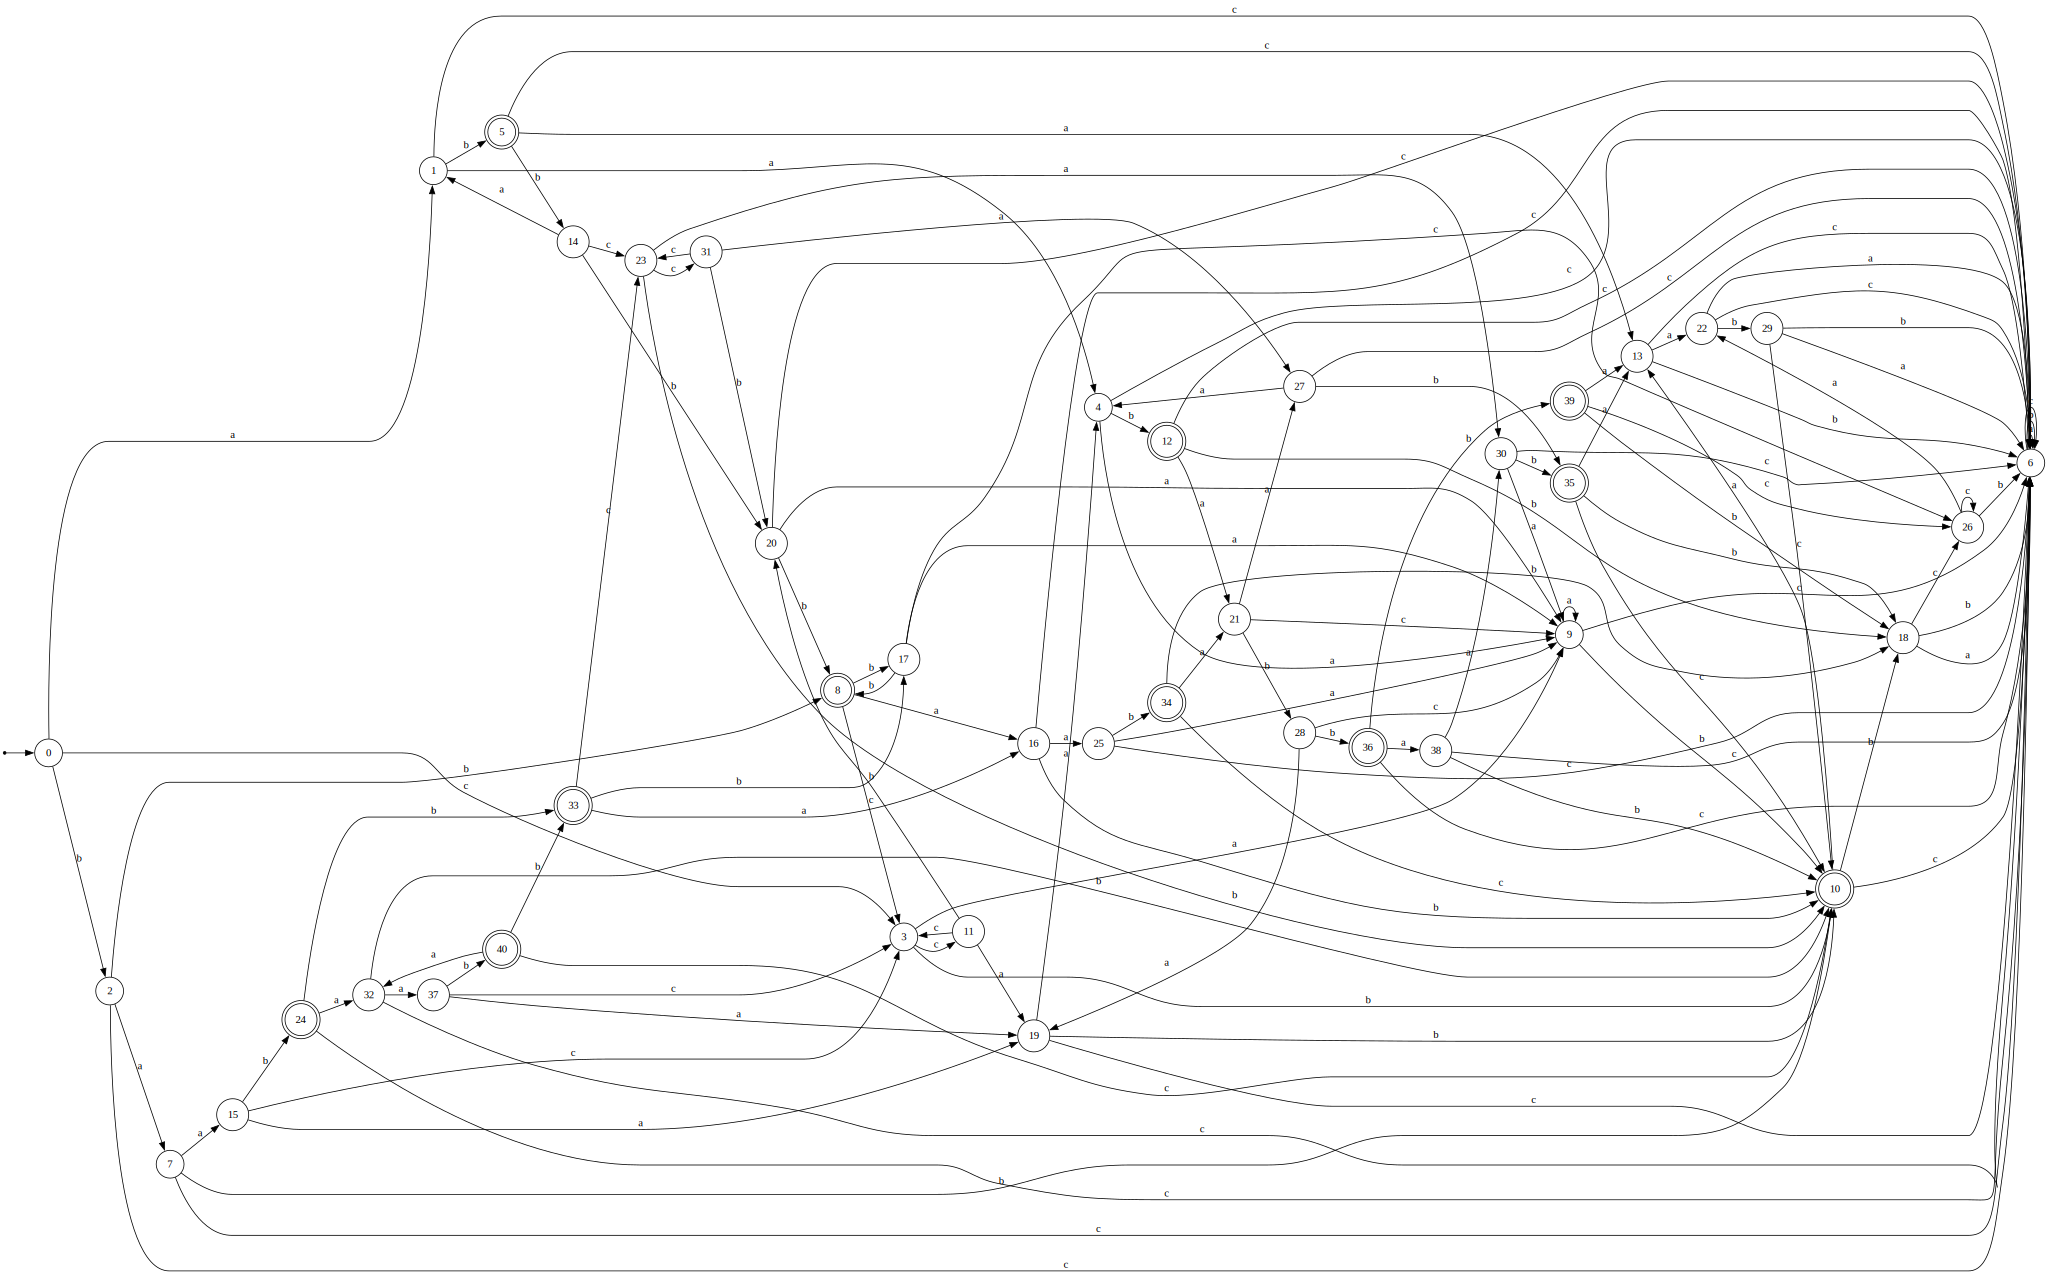
\includegraphics[width=\textwidth]{dka.png}
\newpage
\small
\begin{tabular}{l*{18}{c}}
\hline
--- & b & c & ab & bb & bc & aab & abb & abc & bab & bbb & cab & aabb & aabc & baab & bbab & cabc & abaab & abbab \\
\hline
q0  & 0 & 0 & 1 & 1 & 0 & 1 & 0 & 0 & 1 & 0 & 1 & 0 & 0 & 1 & 1 & 0 & 0 & 1 \\
q1  & 1 & 0 & 1 & 0 & 0 & 1 & 0 & 0 & 0 & 0 & 0 & 0 & 0 & 0 & 1 & 0 & 1 & 0 \\
q2  & 1 & 0 & 1 & 0 & 0 & 1 & 0 & 0 & 1 & 1 & 0 & 1 & 0 & 1 & 1 & 0 & 0 & 0 \\
q3  & 1 & 0 & 1 & 0 & 0 & 1 & 0 & 0 & 0 & 0 & 1 & 0 & 0 & 0 & 0 & 0 & 0 & 0 \\
q4  & 1 & 0 & 1 & 0 & 0 & 1 & 0 & 0 & 0 & 0 & 0 & 0 & 0 & 1 & 0 & 0 & 0 & 0 \\
q5  & 0 & 0 & 0 & 0 & 0 & 0 & 0 & 0 & 1 & 1 & 0 & 0 & 1 & 1 & 1 & 0 & 0 & 0 \\
q6  & 0 & 0 & 0 & 0 & 0 & 0 & 0 & 0 & 0 & 0 & 0 & 0 & 0 & 0 & 0 & 0 & 0 & 0 \\
q7  & 1 & 0 & 1 & 0 & 0 & 1 & 1 & 0 & 0 & 0 & 0 & 0 & 0 & 0 & 0 & 0 & 1 & 1 \\
q8  & 0 & 0 & 1 & 1 & 0 & 1 & 0 & 0 & 1 & 0 & 1 & 0 & 1 & 1 & 1 & 0 & 0 & 0 \\
q9  & 1 & 0 & 1 & 0 & 0 & 1 & 0 & 0 & 0 & 0 & 0 & 0 & 0 & 0 & 0 & 0 & 0 & 0 \\
q10 & 0 & 0 & 0 & 0 & 0 & 0 & 0 & 0 & 0 & 0 & 0 & 0 & 1 & 0 & 0 & 0 & 0 & 0 \\
q11 & 0 & 0 & 1 & 1 & 0 & 1 & 0 & 0 & 1 & 0 & 1 & 0 & 0 & 1 & 1 & 0 & 0 & 0 \\
q12 & 0 & 0 & 0 & 0 & 0 & 1 & 1 & 0 & 0 & 0 & 0 & 0 & 1 & 0 & 0 & 0 & 1 & 1 \\
q13 & 0 & 0 & 0 & 0 & 0 & 0 & 0 & 1 & 0 & 0 & 0 & 0 & 0 & 0 & 0 & 0 & 0 & 0 \\
q14 & 0 & 0 & 1 & 1 & 0 & 1 & 0 & 0 & 1 & 0 & 1 & 0 & 0 & 1 & 1 & 1 & 0 & 1 \\
q15 & 1 & 0 & 1 & 1 & 0 & 1 & 0 & 0 & 1 & 0 & 1 & 0 & 0 & 1 & 1 & 0 & 0 & 0 \\
q16 & 1 & 0 & 1 & 0 & 0 & 1 & 0 & 1 & 0 & 0 & 0 & 0 & 0 & 0 & 0 & 0 & 1 & 0 \\
q17 & 1 & 0 & 1 & 0 & 0 & 1 & 0 & 0 & 1 & 1 & 0 & 0 & 0 & 1 & 1 & 1 & 0 & 0 \\
q18 & 0 & 0 & 0 & 0 & 0 & 0 & 0 & 0 & 0 & 0 & 0 & 0 & 0 & 0 & 0 & 1 & 0 & 0 \\
q19 & 1 & 0 & 1 & 0 & 0 & 1 & 0 & 0 & 0 & 0 & 0 & 0 & 0 & 0 & 0 & 0 & 1 & 0 \\
q20 & 1 & 0 & 1 & 0 & 0 & 1 & 0 & 0 & 1 & 1 & 0 & 0 & 0 & 1 & 1 & 0 & 0 & 0 \\
q21 & 0 & 0 & 1 & 1 & 0 & 1 & 0 & 1 & 1 & 1 & 1 & 0 & 0 & 1 & 1 & 0 & 0 & 0 \\
q22 & 0 & 0 & 0 & 0 & 1 & 0 & 0 & 0 & 0 & 0 & 0 & 0 & 0 & 0 & 0 & 0 & 0 & 0 \\
q23 & 1 & 0 & 1 & 0 & 0 & 1 & 0 & 1 & 0 & 0 & 1 & 0 & 0 & 0 & 0 & 1 & 0 & 0 \\
q24 & 1 & 0 & 1 & 0 & 0 & 1 & 0 & 0 & 1 & 1 & 0 & 1 & 1 & 1 & 1 & 0 & 0 & 0 \\
q25 & 1 & 0 & 1 & 0 & 1 & 1 & 0 & 0 & 0 & 0 & 0 & 0 & 0 & 1 & 0 & 0 & 0 & 0 \\
q26 & 0 & 0 & 0 & 0 & 0 & 0 & 0 & 1 & 0 & 0 & 0 & 0 & 0 & 0 & 0 & 1 & 0 & 0 \\
q27 & 1 & 0 & 1 & 0 & 1 & 1 & 0 & 0 & 0 & 0 & 0 & 0 & 0 & 0 & 0 & 0 & 1 & 0 \\
q28 & 1 & 0 & 1 & 1 & 0 & 1 & 0 & 0 & 1 & 0 & 1 & 0 & 0 & 1 & 0 & 0 & 0 & 0 \\
q29 & 0 & 1 & 0 & 0 & 0 & 0 & 0 & 0 & 0 & 0 & 0 & 0 & 0 & 0 & 0 & 0 & 0 & 0 \\
q30 & 1 & 0 & 1 & 0 & 1 & 1 & 0 & 0 & 0 & 0 & 0 & 0 & 0 & 0 & 0 & 0 & 0 & 0 \\
q31 & 0 & 0 & 1 & 1 & 0 & 1 & 0 & 1 & 1 & 0 & 1 & 0 & 0 & 1 & 1 & 1 & 0 & 0 \\
q32 & 1 & 0 & 1 & 0 & 0 & 1 & 1 & 1 & 0 & 0 & 0 & 0 & 0 & 0 & 0 & 0 & 1 & 1 \\
q33 & 0 & 0 & 1 & 1 & 0 & 1 & 0 & 0 & 1 & 0 & 1 & 0 & 1 & 1 & 1 & 1 & 0 & 0 \\
q34 & 0 & 1 & 0 & 0 & 0 & 1 & 1 & 0 & 0 & 0 & 0 & 0 & 1 & 0 & 0 & 0 & 1 & 1 \\
q35 & 0 & 1 & 0 & 0 & 0 & 0 & 0 & 0 & 0 & 0 & 0 & 0 & 1 & 0 & 0 & 0 & 0 & 0 \\
q36 & 1 & 0 & 1 & 0 & 0 & 1 & 0 & 0 & 0 & 0 & 0 & 0 & 1 & 0 & 0 & 0 & 0 & 0 \\
q37 & 1 & 0 & 1 & 1 & 1 & 1 & 0 & 0 & 1 & 0 & 1 & 0 & 0 & 1 & 1 & 0 & 0 & 0 \\
q38 & 1 & 0 & 1 & 0 & 0 & 1 & 0 & 1 & 0 & 0 & 0 & 0 & 0 & 0 & 0 & 0 & 0 & 0 \\
q39 & 0 & 0 & 0 & 0 & 0 & 0 & 0 & 0 & 0 & 0 & 0 & 0 & 1 & 0 & 0 & 1 & 0 & 0 \\
q40 & 1 & 1 & 1 & 0 & 0 & 1 & 0 & 0 & 1 & 1 & 0 & 1 & 1 & 1 & 1 & 0 & 0 & 0 \\
\hline
\end{tabular}
\label{tab:states}
\newline

\section*{Возможно малый ПКА}
\includegraphics[width=\textwidth]{pka.png}
\begin{table}[h]
\centering
\normalsize
\begin{tabular}{l*{3}{c}}
\hline
      & E & bb & ab \\
\hline
E     & 0 & 1  & 1  \\
a     & 0 & 0  & 1  \\
b     & 0 & 0  & 0  \\
\hline
\end{tabular}
\label{tab:prefix2}
\end{table}

\section*{Расширенное регулярное выражение}
\[
\textasciicircum(((baa)+)?|((abb)+)?)((bb|cc)+)?((aaba(b)?)+)?.(a+)?b(((a|bc+)abc)+)?\$
\]
\end{document}

